\documentclass[tikz,border=10pt]{standalone}
\usetikzlibrary{calc}

\begin{document}
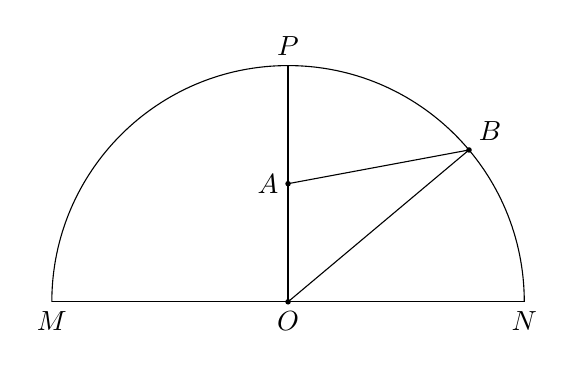
\begin{tikzpicture}
    % --- 参数定义 ---
    \def\R{3} % 半圆半径
    
    % --- 定义坐标 ---
    \coordinate (O) at (0,0);
    \coordinate (M) at (-\R,0);
    \coordinate (N) at (\R,0);
    \coordinate (P) at (0,\R);
    % 设置点 A 在 OP 上 (0.5 为从 O 到 P 的比例)
    \coordinate (A) at (0, 0.5*\R); 
    % 设置点 B 在圆弧上 (定义角度为 40 度)
    \coordinate (B) at (40:\R);
    
    % --- 绘制图形 ---
    % 绘制底边 MN
    \draw (M) -- (N);
    % 绘制半圆弧
    \draw (M) arc (180:0:\R);
    % 绘制半径 OP
    \draw (O) -- (P);
    % 绘制线段 AB 和 OB
    \draw (A) -- (B) -- (O);
    
    % --- 标注点 ---
    \node[below] at (M) {$M$};
    \node[below] at (N) {$N$};
    \node[below] at (O) {$O$};
    \node[above] at (P) {$P$};
    \node[left] at (A) {$A$};
    \node[above right] at (B) {$B$};
    
    % --- 可选：标记点 ---
    \fill (O) circle (1pt);
    \fill (A) circle (1pt);
    \fill (B) circle (1pt);

\end{tikzpicture}
\end{document}